\documentclass{article}

\usepackage{titlesec}

\usepackage{amsmath}
\usepackage{amssymb}

\usepackage{booktabs}
\usepackage{float}
\usepackage{colortbl}
\usepackage{xcolor}

\usepackage{a4wide}
\usepackage{setspace}
\usepackage{geometry}
\usepackage{parskip}

\usepackage{multirow}
\usepackage{adjustbox}
\usepackage{graphicx}

\usepackage{hyperref}
\hypersetup{
    colorlinks=true,
    linkcolor=black,
    urlcolor=blue
}

\DeclareRobustCommand{\bbone}{\text{\usefont{U}{bbold}{m}{n}1}}

\titleformat*{\subsection}{\normalfont}

\author{Yu Xia \\ ID: yx5262}
\title{Yu Xia's Answer for Problem Set 7}
\date{Fall 2022}

\begin{document}
\maketitle

\nocite{*}

\section*{1}

\begin{figure}[H]
    \begin{center}
        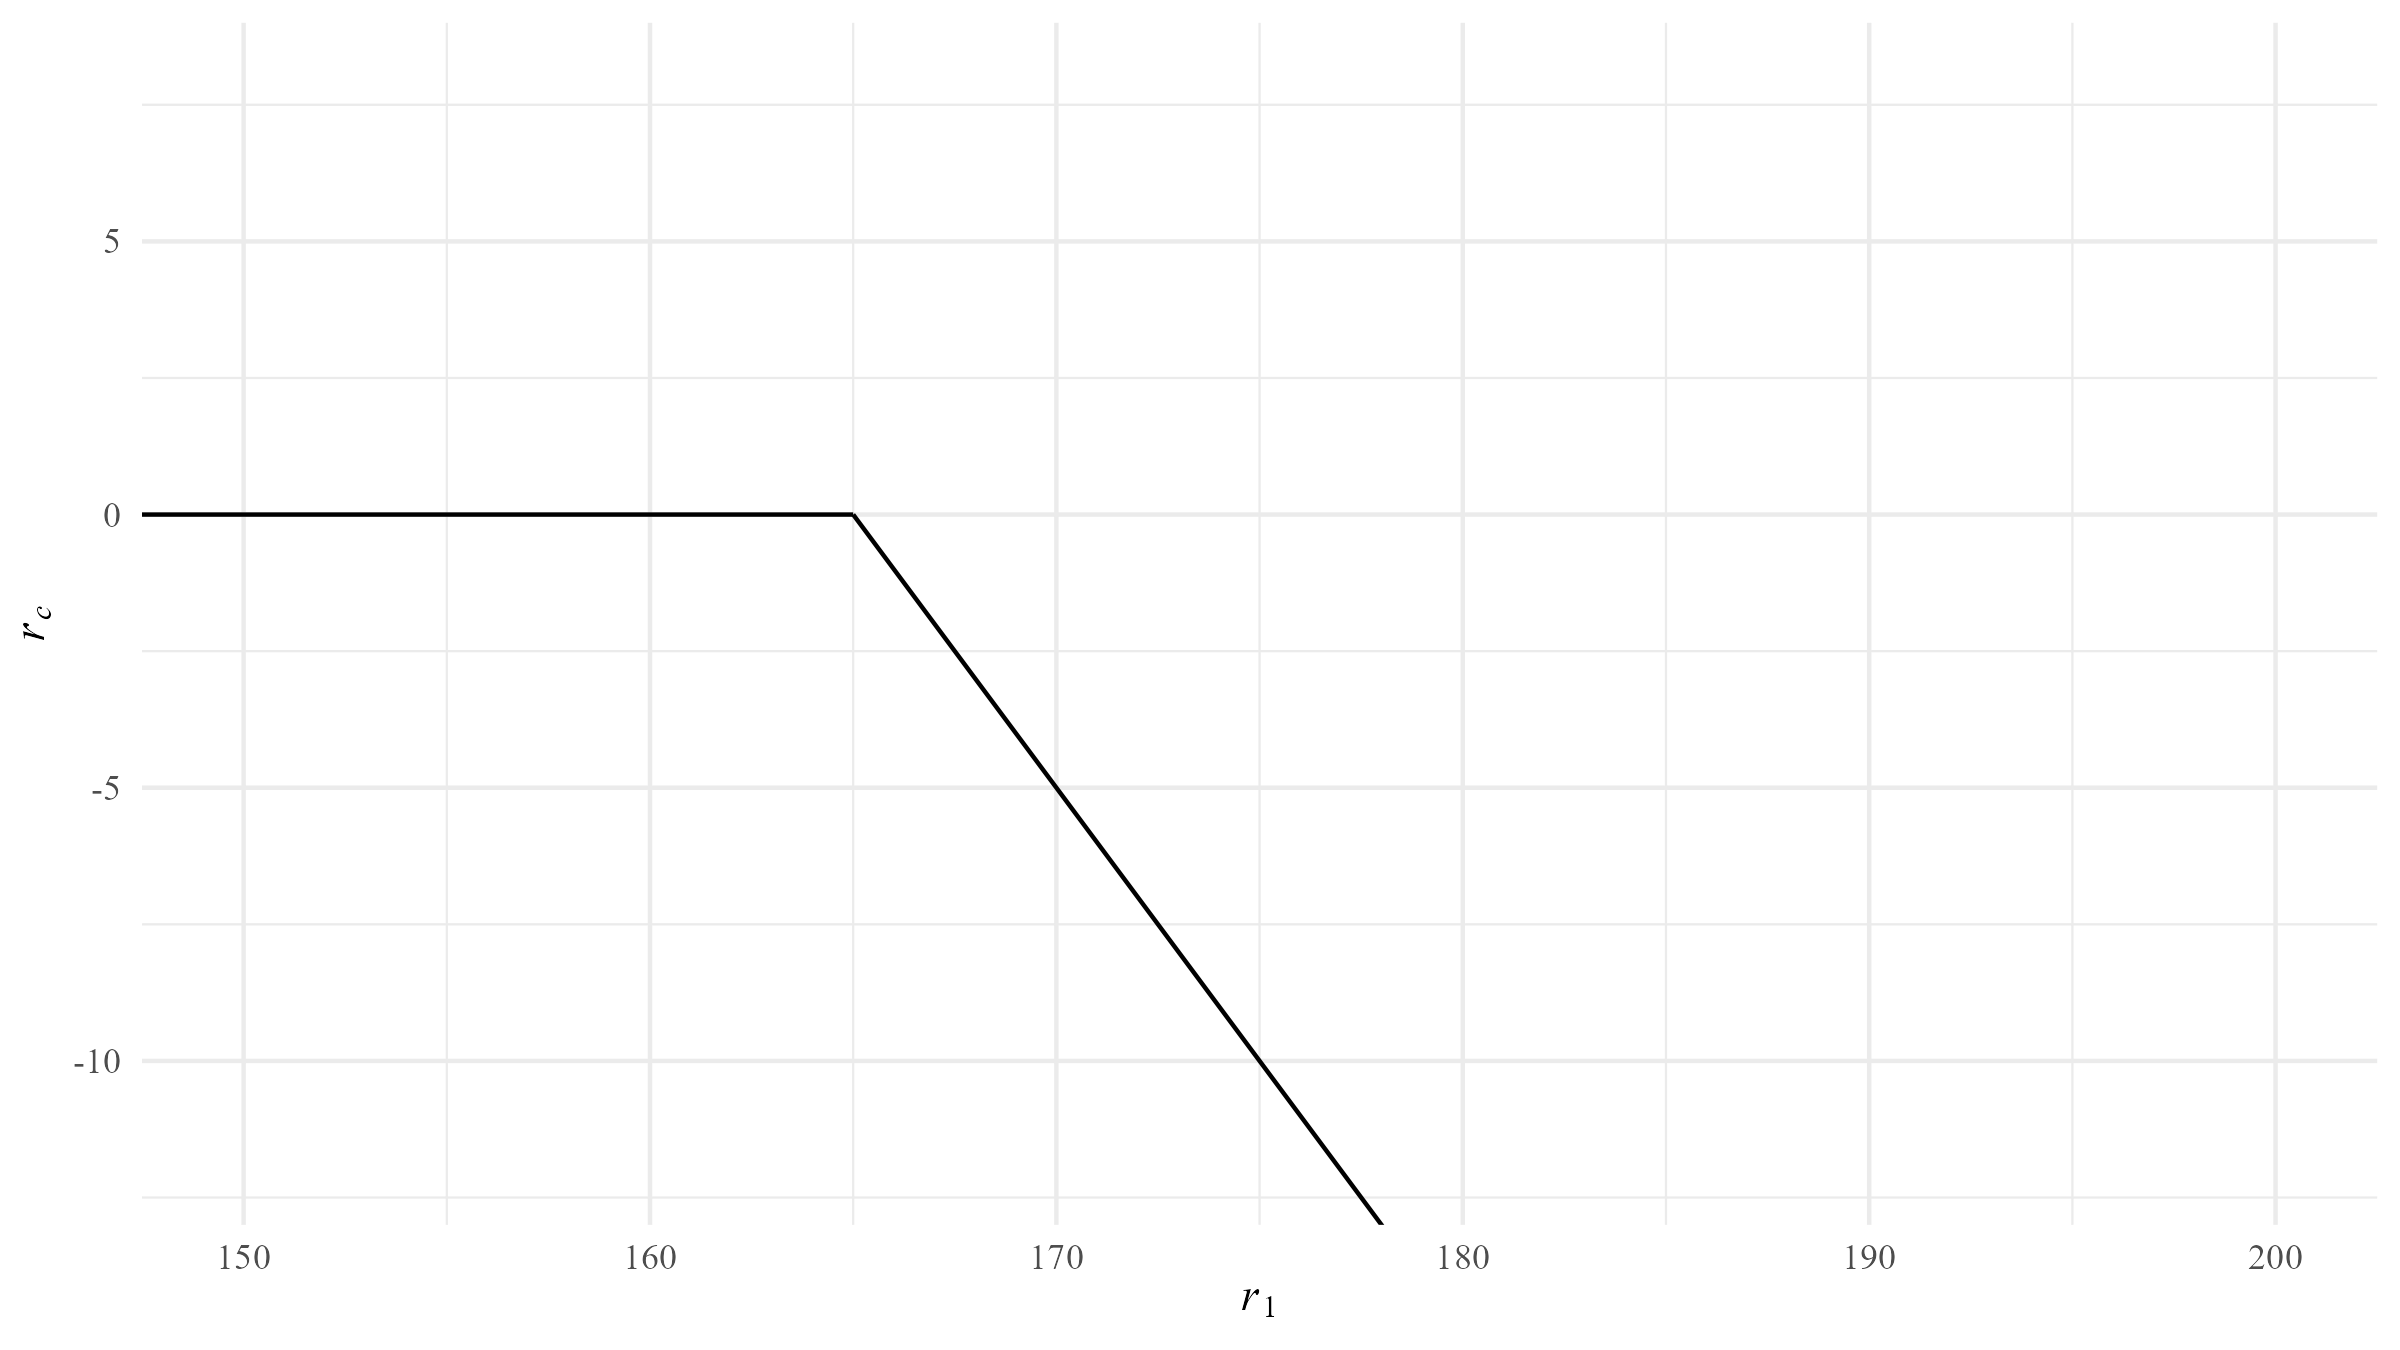
\includegraphics[width=1\textwidth]{figures/PS7a1.png}
    \end{center}
    \caption{Payoff from short position in the European call with the strike \$165}
    \label{fig:graph}
\end{figure}

\begin{figure}[H]
    \begin{center}
        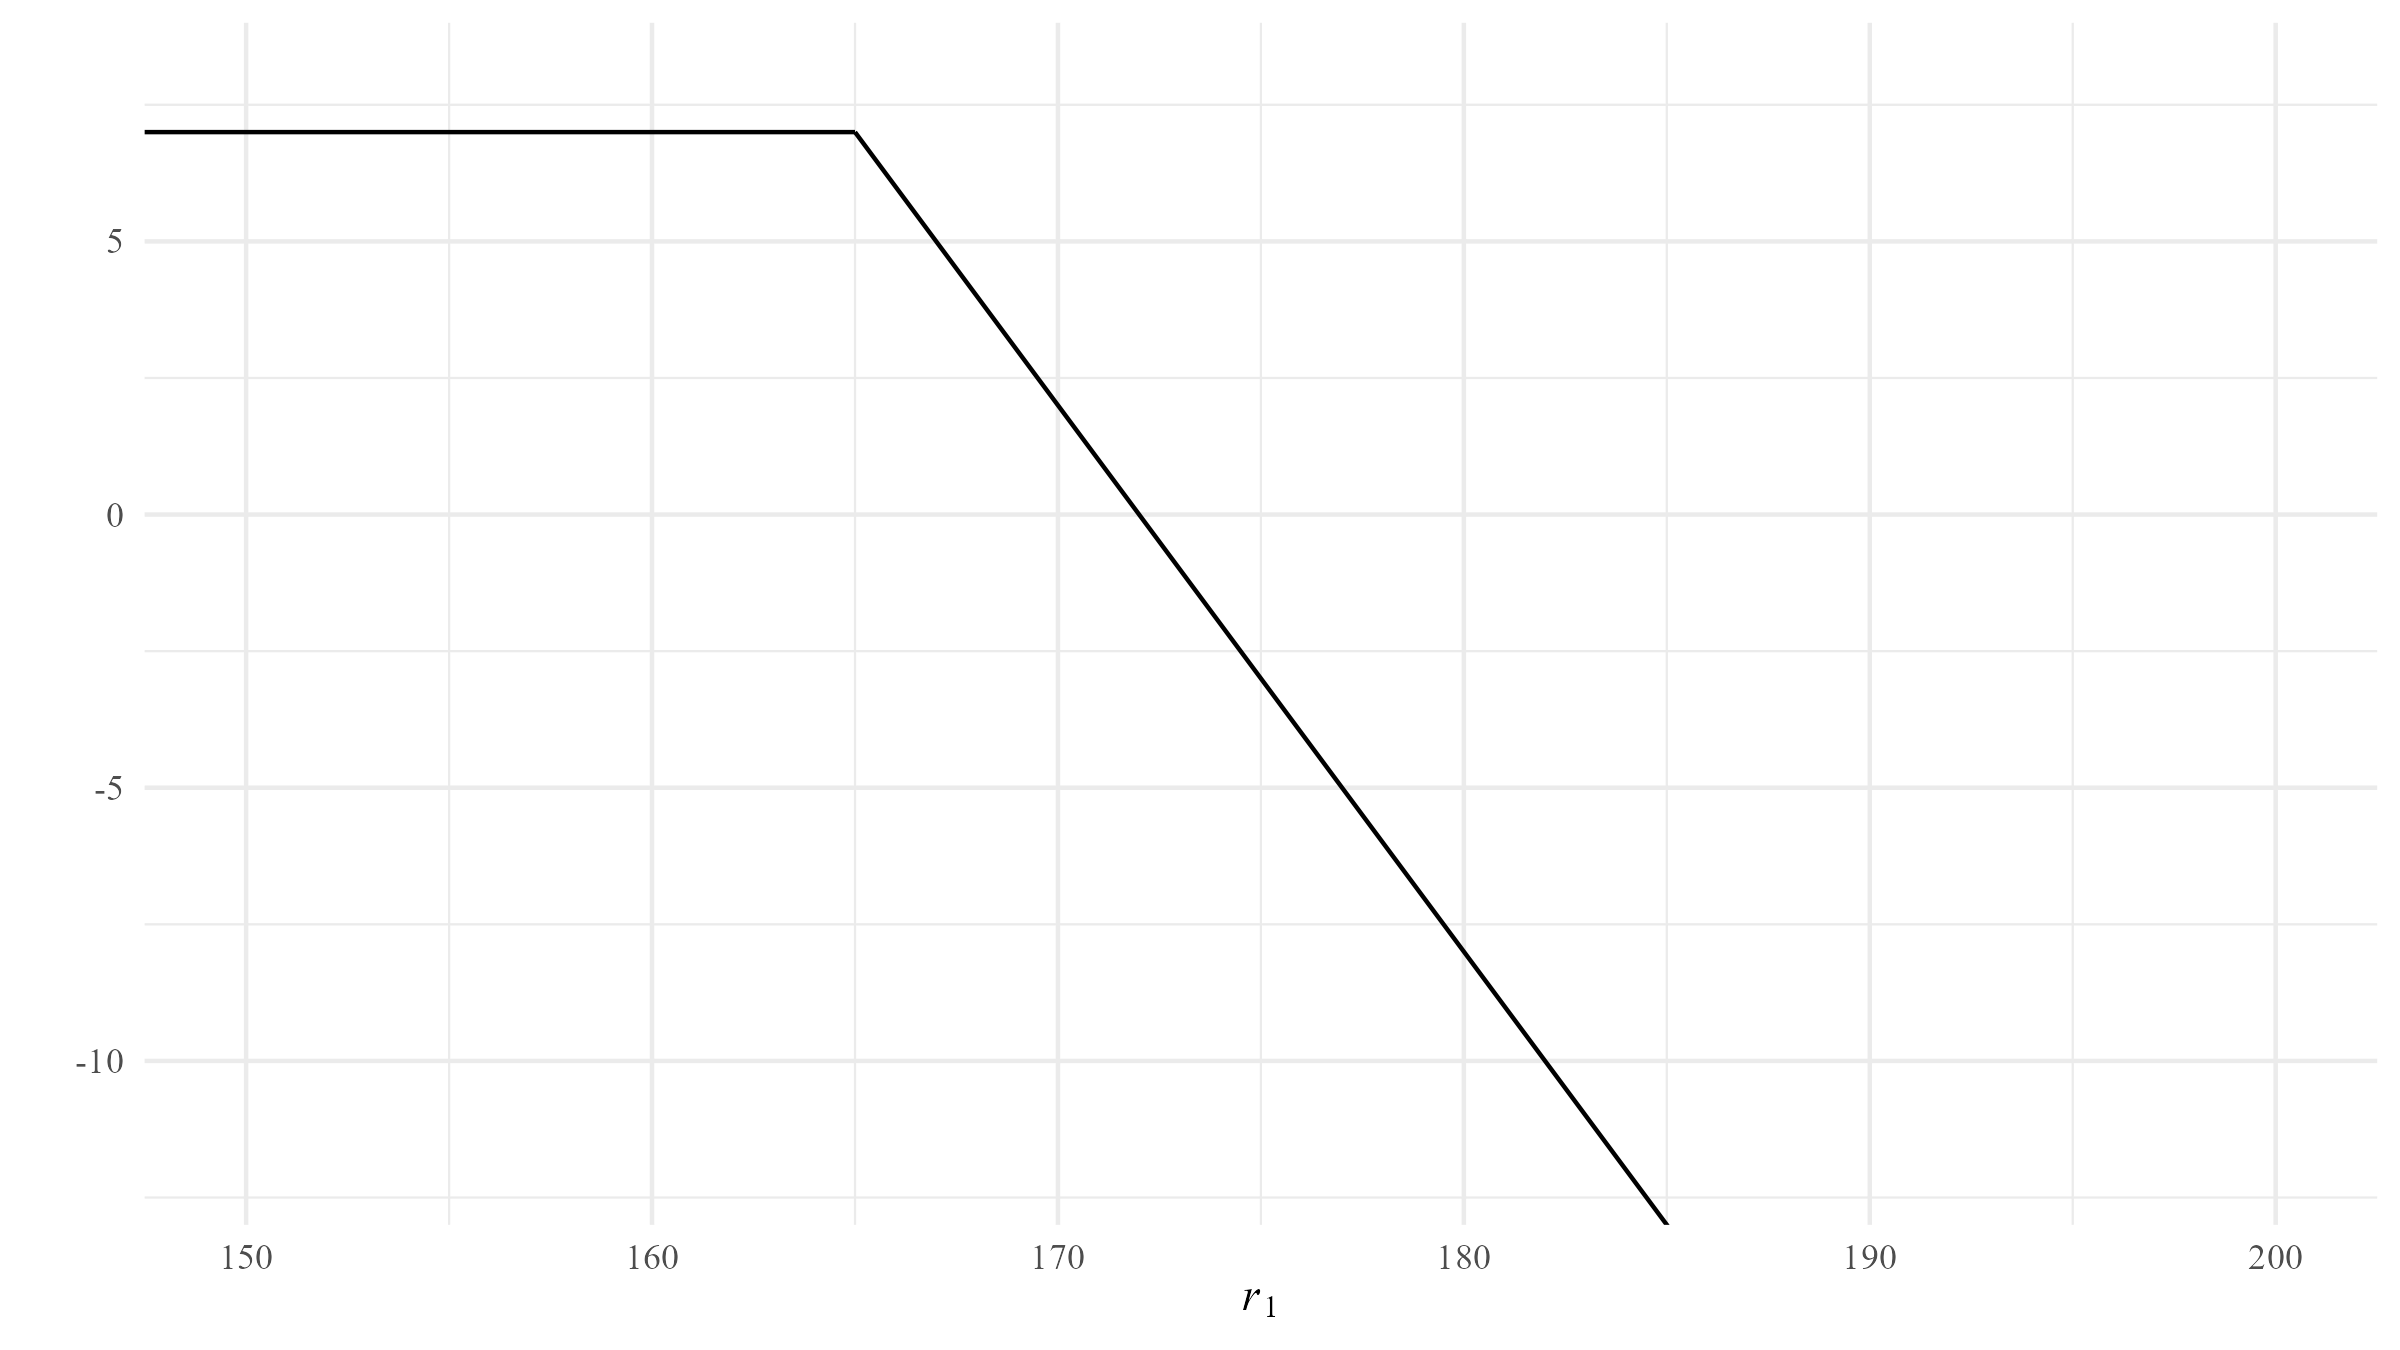
\includegraphics[width=1\textwidth]{figures/PS7a2.png}
    \end{center}
    \caption{Profit from short position in the European call with the strike \$165 and spot price \$7}
    \label{fig:graph}
\end{figure}

\begin{figure}[H]
    \begin{center}
        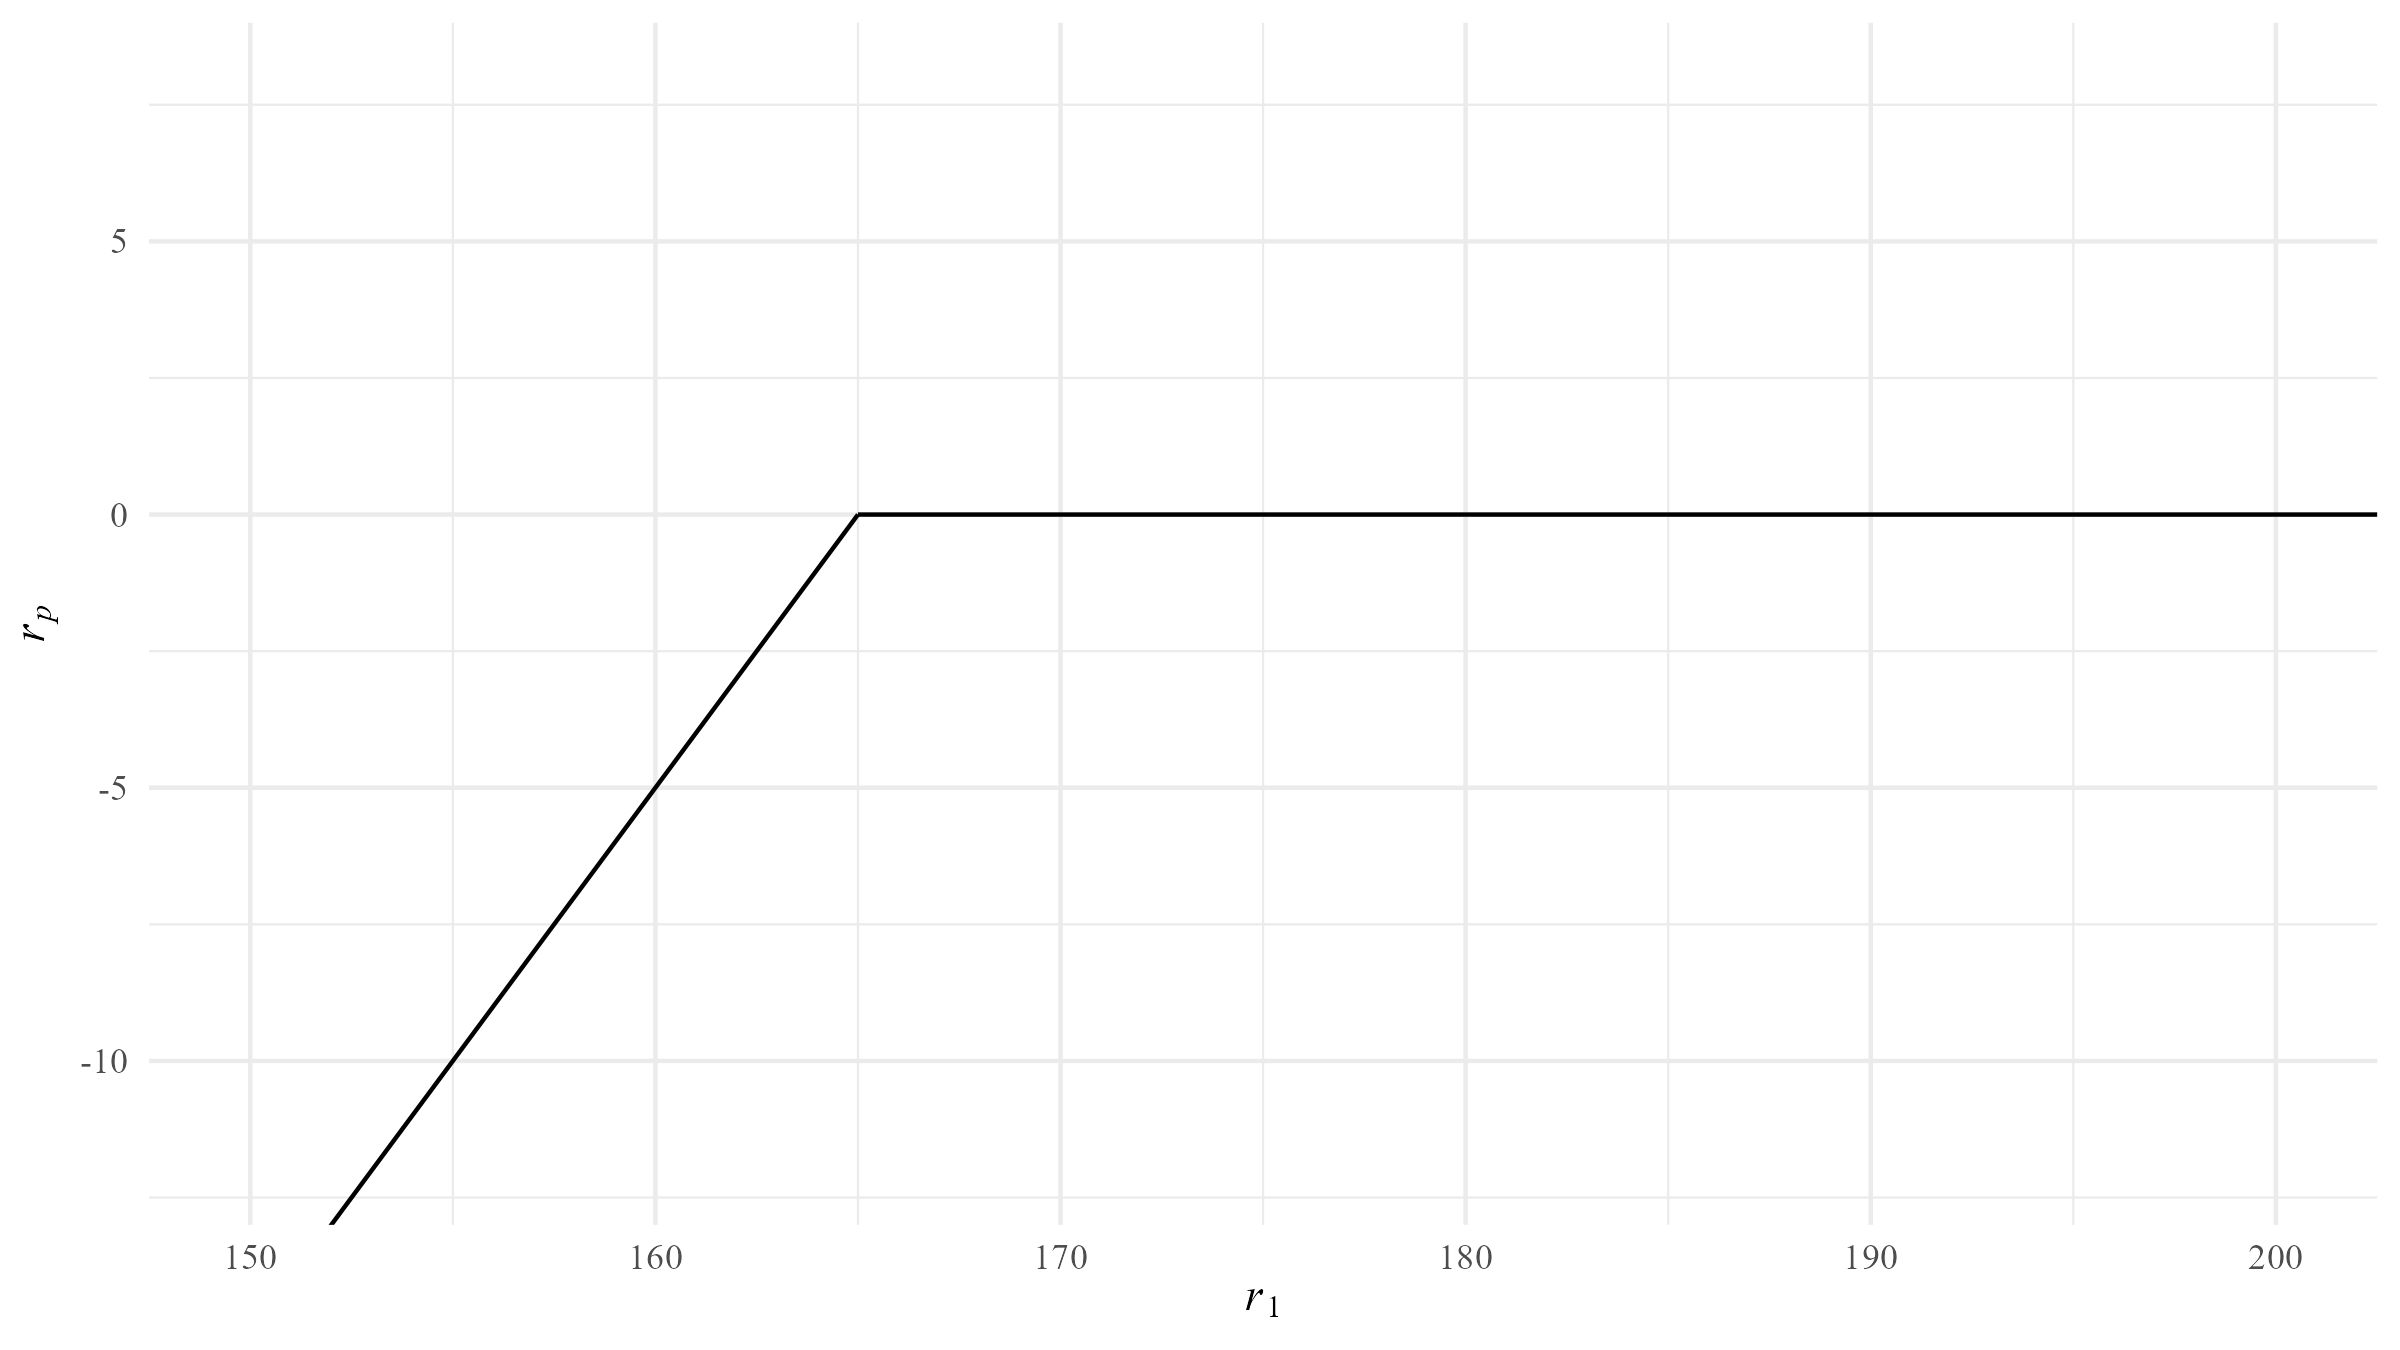
\includegraphics[width=1\textwidth]{figures/PS7a3.png}
    \end{center}
    \caption{Payoff from short position in the European put with the strike \$165}
    \label{fig:graph}
\end{figure}

\begin{figure}[H]
    \begin{center}
        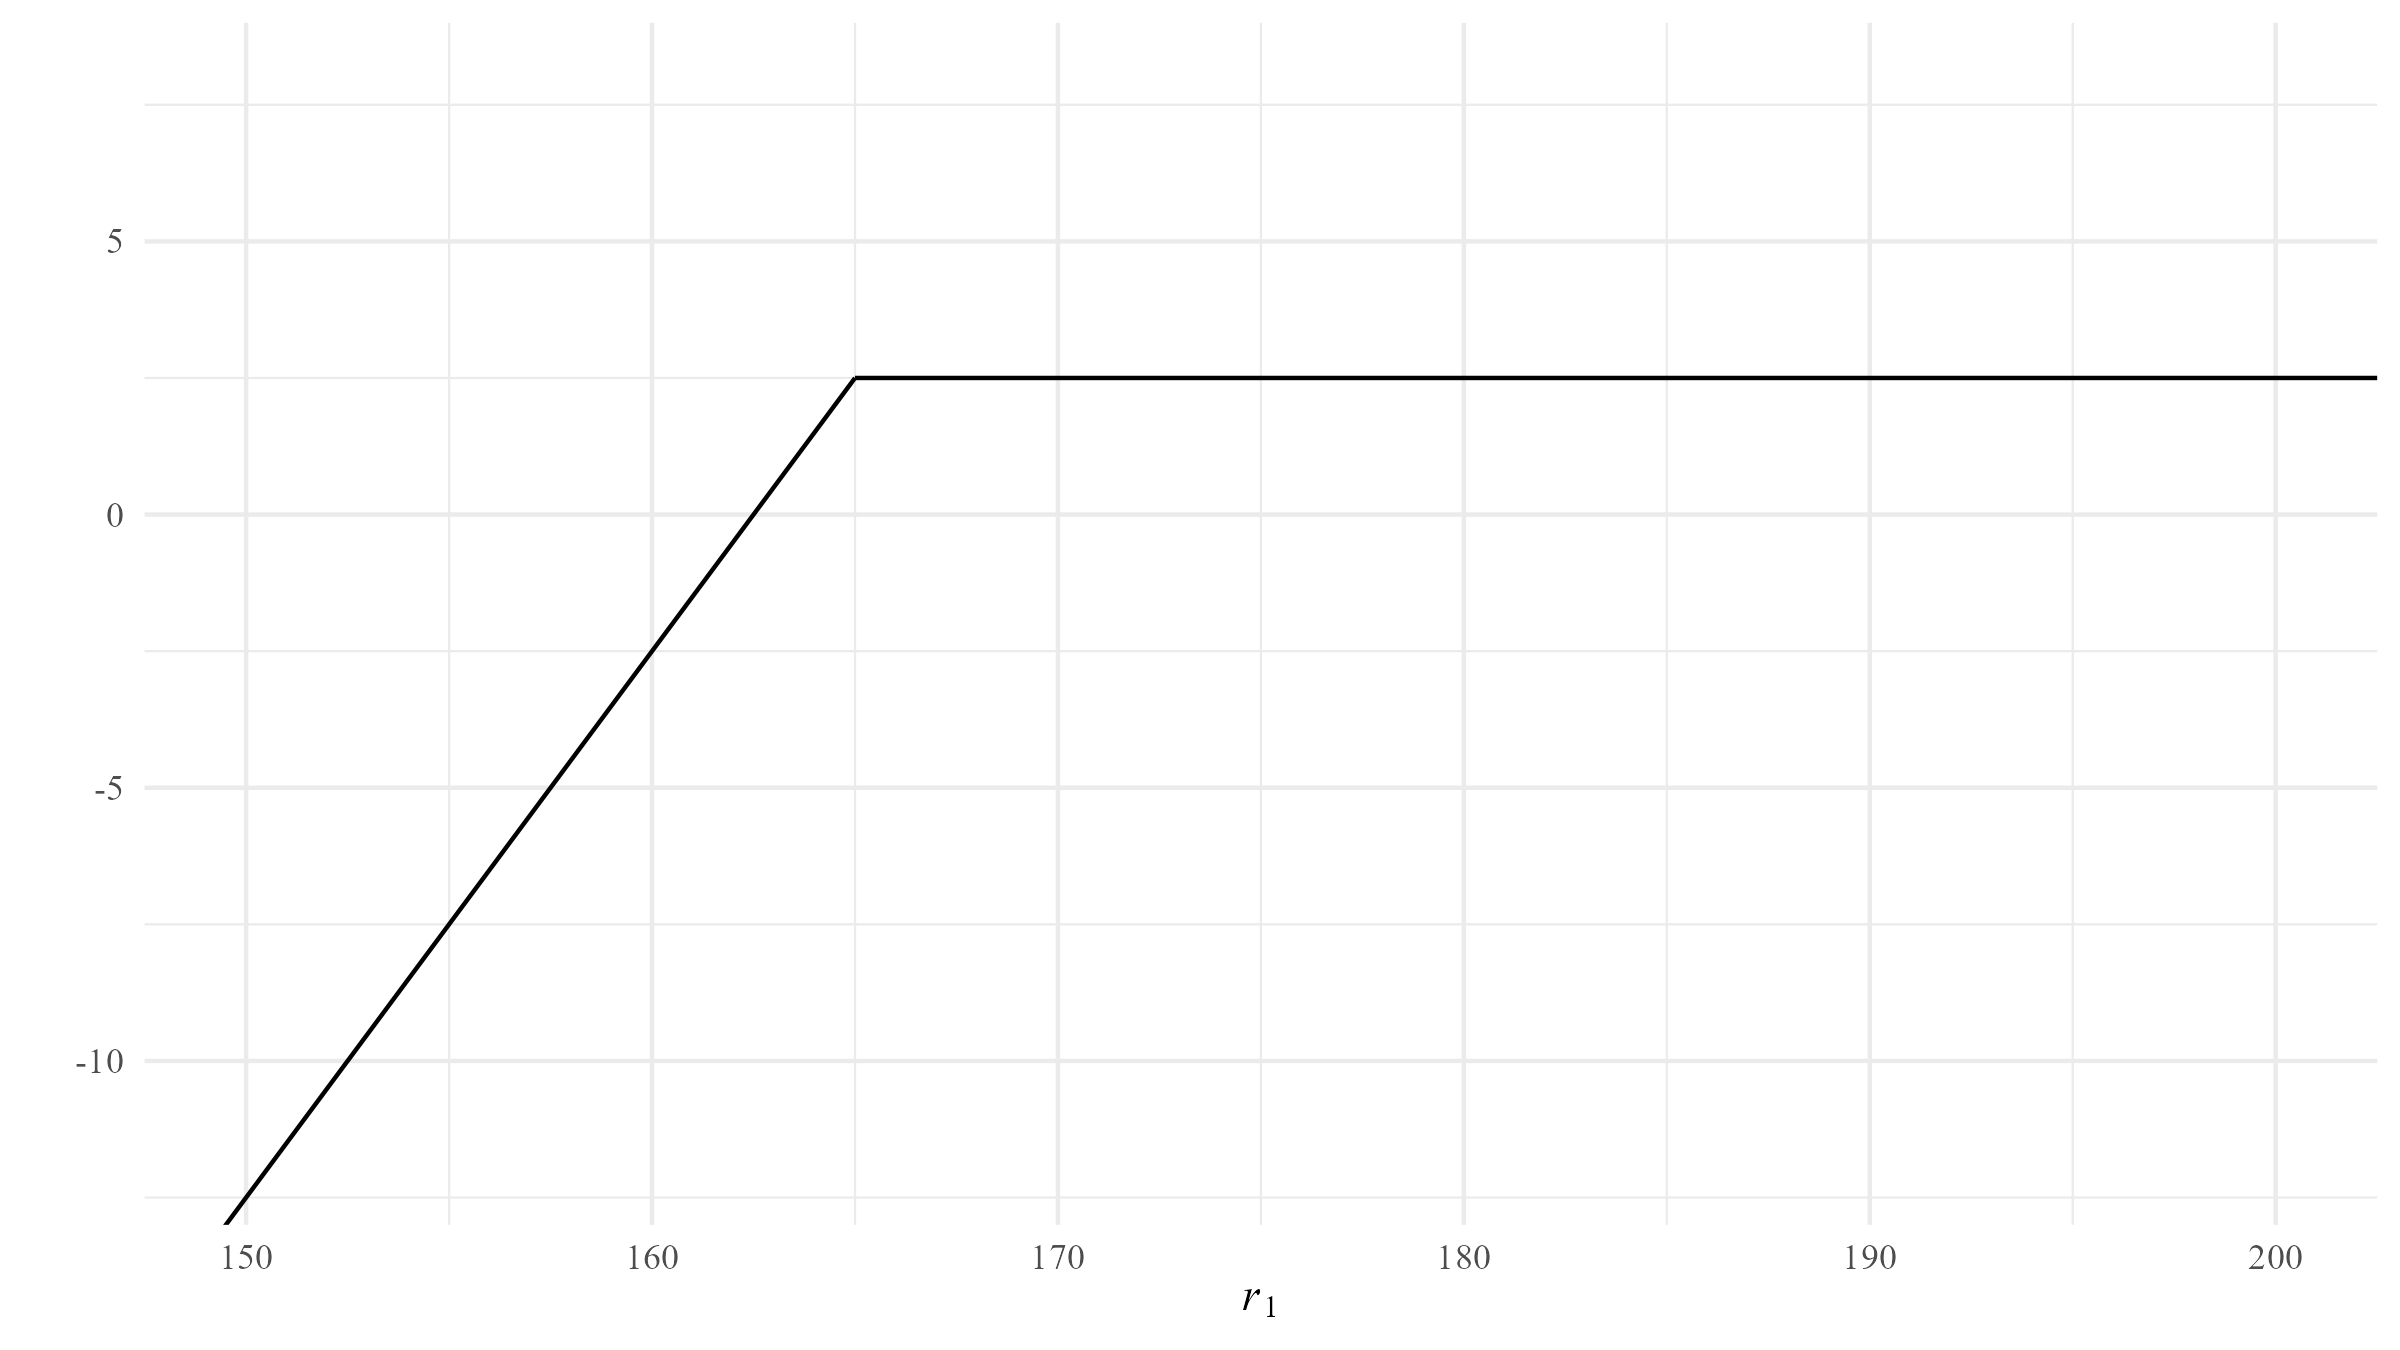
\includegraphics[width=1\textwidth]{figures/PS7a4.png}
    \end{center}
    \caption{Profit from short position in the European put with the strike \$165 and spot price \$7}
    \label{fig:graph}
\end{figure}


\section*{2}

\subsection*{(a)}

Denote the probability of increasing stock price as $\pi$. Thus the probability measure is $\left\{\pi, 1-\pi\right\}$.

$60=\dfrac{1}{1.002}\left(80\pi+30\left(1-\pi\right)\right)=\dfrac{1}{1.002}\left(80\pi+30-30\pi\right)=\dfrac{1}{1.002}\left(50\pi+30\right)$

$\implies 50\pi+30=60\times1.002=60.12\implies50\pi=30.12\implies5\pi=3.012\implies10\pi=6.024$

$\implies\pi=0.6024$

$\therefore$ The probability measure is $\boxed{\left\{0.6024, 0.3976\right\}}$.

\subsection*{(b)}

Denote this portfolio consists of $\alpha_{c}$ shares of the stock and $\beta_{c}$ shares of the bond.

If $q_{1}=80>40=K$, investor exercises, and the payoff is $80-40=40$.

If $q_{1}=30<40=K$, investor won't exercise, the payoff is $0$. 

\begin{align*} 
    80\alpha_{c} + 1.002\beta_{c} &=  40 \\ 
    30\alpha_{c} + 1.002\beta_{c} &=  0
\end{align*}

$\implies 50\alpha_{c}=40\implies\alpha_{c}=0.8$

$1.002\beta_{c}=-30\alpha_{c}=-30\times0.8=-24\implies\beta_{c}=\dfrac{-24}{1.002}=\dfrac{-12}{0.501}\approx-23.952$

Hence the European call can be replicated by buying $0.8$ shares of the stock and shorting $23.952$ shares of the bond.

\subsection*{(c)}

In an economy, there are $S$ Arrow securities, $K<S$ other assets. The payoff matrix of assets is:

\begin{equation*}
    R=\begin{pmatrix}
        r_{11} & \dots & r_{1k} & \dots & r_{1K} \\
        \vdots & \ddots & \vdots & \ddots & \vdots\\
        r_{s1} & \dots & r_{sk} & \dots & r_{sK} \\
        \vdots & \ddots & \vdots & \ddots & \vdots\\
        r_{S1} & \dots & r_{Sk} & \dots & r_{SK}
    \end{pmatrix}
\end{equation*}

$\lambda_{s}$ denotes the price of Arrow security in state $s$, $q_{k}$ denotes the spot price of asset $k$.

Then the no-arbitrage price of asset $k$ is 

\begin{equation*}
    q_{k}=\lambda r_{k}=\sum^{S}_{s=1}\lambda_{s}r_{sk}
\end{equation*}

The investor cannot make profit out of nothing, given the arbitrage free price system.

The price in this problem is:

$q_{c}\approx0.8\times\$60-\$23.952\approx\$48-\$23.952\approx\boxed{\$24.0479}$

\subsection*{(d)}

Suppose that $q_{c}<\$24.0479$.

Consider a portfolio consisting of $1$ share of call option, $\alpha_{c}=0.8$ shares of stock, and $\beta_{c}=-23.952$ shares of bond.

The market value of the portfolio is:

$q_{c}-60\alpha_{c}-\beta_{c}<0$

Suppose $q_{1}=\$80$, then the investor exercises the call, getting $\$40$, and also gets back $\$1.002\times23.952=\$24$ on the bond holding.

$\therefore$ The investor's payment ends up $\$40+\$24=\$64$.

This investor uses these payments to buy $\alpha_{c}=0.8$ shares of stock at $\$80$ and pays back the debt.

Since $0.8\times\$80=\$64$, the net payoff on the portfolio is $0$.

If $q_{1}=\$30$, investor doesn't exercise the call, using the payment of $\$1.002\times23.952=\$24$ to buy $\alpha_{c}=0.8$ shares of stock at $\$30$ and pays back the debt.

Since $0.8\times\$30=\$24$, the net payoff on the portfolio is $0$.

The case when $q_{c}-60\alpha_{c}-\beta_{c}>0$ is similar.

\section*{3}

\subsection*{(b)}

Denote this portfolio consists of $\alpha_{p}$ shares of the stock and $\beta_{p}$ shares of the bond.

If $q_{1}=80>40=K$, investor won't exercise, the payoff is $0$.

If $q_{1}=30<40=K$, investor exercises, and the payoff is $40-30=10$. 

\begin{align*} 
    80\alpha_{p} + 1.002\beta_{p} &=  0 \\ 
    30\alpha_{p} + 1.002\beta_{p} &=  10
\end{align*}

$\implies 50\alpha_{p}=-10\implies\alpha_{p}=-0.2$

$1.002\beta_{p}=-80\alpha_{p}=80\times0.2=8\times2=16\implies\beta_{p}=\dfrac{16}{1.002}=\dfrac{8}{0.501}\approx15.968$

Hence the European pull can be replicated by shorting $0.2$ shares of the stock and buying $15.968$ shares of the bond.

\subsection*{(d)}

The price

$q_{p}\approx-0.2\times\$60+\$15.968\approx-2\times\$6+\$15.968\approx-\$12+\$15.968\approx\$3.968$

Suppose that $q_{c}<\$3.968$.

Consider a portfolio consisting of $1$ share of call option, $\alpha_{c}=-0.2$ shares of stock, and $\beta_{c}=15.968$ shares of bond.

The market value of the portfolio is:

$q_{c}-60\alpha_{c}-\beta_{c}<0$

If $q_{1}=\$80$, investor doesn't exercise the put, sell $0.2$ shares of the stock, getting $0.2\times\$80=2\times\$8=\$16$, and using the money to pay back my debt $\$1.002\times15.968=\$16$.

The net payoff on the portfolio is $0$.

Suppose $q_{1}=\$30$, then the investor exercises the put, getting $\$10$, and also sells $0.2$ of the stock, getting $0.2\times\$30=2\times\$3=\$6$.

Use this money to pay back the debt of the bond $\$1.002\times15.968=\$16$.

$\therefore$ Net payoff on the portfolio is $0$.

The case when $q_{c}-60\alpha_{c}-\beta_{c}>0$ is similar.

\section*{4}

\subsection*{(a)}

Denote the probability of increasing stock price as $\pi$. Thus the probability measure is $\left\{\pi, 1-\pi\right\}$.

$q_{0}=\dfrac{1}{1+r}\left(q_{H}\pi+q_{L}\left(1-\pi\right)\right)$

$\implies \dfrac{1}{1+r}\left(q_{L}\pi+q_{L}\left(1-\pi\right)\right)\leqslant q_{0}\leqslant\dfrac{1}{1+r}\left(q_{H}\pi+q_{H}\left(1-\pi\right)\right)$

$\implies \boxed{\dfrac{q_{L}}{1+r}\leqslant q_{0}\leqslant\dfrac{q_{H}}{1+r}}$

For the call option:

$q_{c}=\dfrac{1}{1+r}\left(\left(q_{H}-K\right)\pi+0\cdot\left(1-\pi\right)\right)=\dfrac{\pi}{1+r}\left(q_{H}-K\right)$

$\implies\pi=\dfrac{q_{c}\left(1+r\right)}{q_{H}-K}$

\subsection*{(b)}

Denote this portfolio consists of $\alpha_{c}$ shares of the stock and $\beta_{c}$ shares of the bond.

If $q_{1}=q_{H}>K$, investor exercises, and the payoff is $q_{H}-K>0$.

If $q_{1}=q_{L}<K$, investor won't exercise, the payoff is $0$. 

\begin{align*} 
    q_{H}\alpha_{c} + \left(1+r\right)\beta_{c} &=  q_{H}-K \\ 
    q_{L}\alpha_{c} + \left(1+r\right)\beta_{c} &=  0
\end{align*}

$\implies \left(q_{H}-q_{L}\right)\alpha_{c}=q_{H}-K\implies\alpha_{c}=\dfrac{q_{H}-K}{q_{H}-q_{L}}$

$\left(1+r\right)\beta_{c}=-q_{L}\alpha_{c}=\dfrac{-q_{L}\left(q_{H}-K\right)}{q_{H}-q_{L}}\implies\beta_{c}=\dfrac{-q_{L}\left(q_{H}-K\right)}{\left(1+r\right)\left(q_{H}-q_{L}\right)}$

Hence the European call can be replicated by buying $\dfrac{q_{H}-K}{q_{H}-q_{L}}$ shares of the stock and shorting $\dfrac{q_{L}\left(q_{H}-K\right)}{\left(1+r\right)\left(q_{H}-q_{L}\right)}$ shares of the bond.

\subsection*{(c)}

$q_{c}=\alpha_{c}q_{0}+\beta_{c}\left(1+r\right)=\dfrac{q_{0}\left(q_{H}-K\right)}{q_{H}-q_{L}}-\dfrac{q_{L}\left(q_{H}-K\right)}{q_{H}-q_{L}}=\dfrac{\left(q_{0}-q_{L}\right)\left(q_{H}-K\right)}{q_{H}-q_{L}}$

Suppose that $q_{c}<\dfrac{\left(q_{0}-q_{L}\right)\left(q_{H}-K\right)}{q_{H}-q_{L}}$.

Consider a portfolio consisting of $1$ share of call option, $\alpha_{c}=\dfrac{q_{H}-K}{q_{H}-q_{L}}$ shares of stock, and $\beta_{c}=\dfrac{-q_{L}\left(q_{H}-K\right)}{\left(1+r\right)\left(q_{H}-q_{L}\right)}$ shares of bond.

The market value of the portfolio is:

$q_{c}-q_{0}\alpha_{c}-\beta_{c}<0$

Suppose $q_{1}=q_{H}$, then the investor exercises the call, getting $q_{H}-K$, and also get back $\left(1+r\right)|\beta_{c}|=\dfrac{q_{L}\left(q_{H}-K\right)}{q_{H}-q_{L}}$ on the bond holding.

$\therefore$ The investor's payment ends up 

$\left(q_{H}-K\right)+\dfrac{q_{L}\left(q_{H}-K\right)}{q_{H}-q_{L}}=\dfrac{\left(q_{H}-q_{L}\right)\left(q_{H}-K\right)}{q_{H}-q_{L}}+\dfrac{q_{L}\left(q_{H}-K\right)}{q_{H}-q_{L}}=\dfrac{q_{H}\left(q_{H}-K\right)}{q_{H}-q_{L}}$.

Investor use these payment to buy $\alpha_{c}=\dfrac{q_{H}-K}{q_{H}-q_{L}}$ shares of stock at $q_{H}$ and pays back the debt.

Since $\alpha_{c}q_{H}=\dfrac{q_{H}\left(q_{H}-K\right)}{q_{H}-q_{L}}$, the net payoff on the portfolio is $0$.

If $q_{1}=q_{L}$, investor doesn't exercise the call, using the payment of $\left(1+r\right)|\beta_{c}|=\dfrac{q_{L}\left(q_{H}-K\right)}{q_{H}-q_{L}}$ to buy $\alpha_{c}=\dfrac{q_{H}-K}{q_{H}-q_{L}}$ shares of stock at $q_{L}$ and pays back the debt.

Since $\alpha_{c}q_{L}=\dfrac{q_{L}\left(q_{H}-K\right)}{q_{H}-q_{L}}$, the net payoff on the portfolio is $0$.

\subsection*{(d)}

$\dfrac{\pi}{1+r}$ in state 1,

$\dfrac{1-\pi}{1+r}$ in state 2.

If plug in the risk-neutral probability:

$\dfrac{q_{c}}{q_{H}-K}$ in state 1,

$1-\pi=1-\dfrac{q_{c}\left(1+r\right)}{q_{H}-K}=\dfrac{q_{H}-K-q_{c}\left(1+r\right)}{q_{H}-K}$

$\dfrac{q_{H}-K-q_{c}\left(1+r\right)}{\left(q_{H}-K\right)\left(1+r\right)}=\dfrac{1}{1+r}-\dfrac{q_{c}}{q_{H}-K}$ in state 2.

\section*{5}

\subsection*{(a)}

Impossible.

Denote this portfolio consists of $\alpha_{p}$ shares of the stock and $\beta_{p}$ shares of the bond.

If $q_{1}=80>40=K$, investor won't exercise, the payoff is $0$.

If $q_{1}=40=K$, investor will be indifferent with whether to exercise or not.

If $q_{1}=30<40=K$, investor exercises, and the payoff is $40-30=10$. 

\begin{align*} 
    80\alpha_{p} + 1.002\beta_{p} &=  0 \\
    40\alpha_{p} + 1.002\beta_{p} &=  0 \\ 
    30\alpha_{p} + 1.002\beta_{p} &=  10
\end{align*}

$\implies 50\alpha_{p}=-10\implies\alpha_{p}=-0.2$

On the other hand, $\left(80-40\right)\alpha_{p}=0$, by subtracting the first 2 equations.

Hence the European pull in this case cannot be replicated.

In other words, since rank$R<K$, cannot be replicated. 

\subsection*{(b)}

The payoff matrix is not in the full rank (or the number of assets is less than the number of states) after simplification, the European pull in this case cannot be replicated by hedging. Thus, it is \textbf{NOT} complete.

\subsection*{(c)}

Denote a risk-neutral probability measure $\left\{\pi_{1}, \pi_{2}, \pi_{3}\right\}$.

By the non-arbitrage equation, for the European put option:

$q_{p}=\dfrac{1}{1+r}\left(0\times\pi_{1}+0\times\pi_{2}+10\pi_{3}\right)=\dfrac{10\pi_{3}}{1.002}\in\left[0,\dfrac{10}{1.002}\right]\approx\left[0,9.98\right]$

For the bond:

$1=\dfrac{1}{1.002}\left(1.002\pi_{1}+1.002\pi_{2}+1.002\pi_{3}\right)\iff\pi_{1}+\pi_{2}+\pi_{3}=1$

On the other hand, for the price of the stock:

$q_{0}=60=\dfrac{1}{1.002}\left(80\pi_{1}+60\pi_{2}+30\pi_{3}\right)$

$\implies60\times1.002=80\pi_{1}+60\left(1-\pi_{1}-\pi_{3}\right)+30\pi_{3}$

$\implies6\times10.02=80\pi_{1}+60-60\pi_{1}-60\pi_{3}+30\pi_{3}$

$\implies60.12=20\pi_{1}+60-30\pi_{3}$

$\implies6.012=6+2\pi_{1}-3\pi_{3}$

$\implies0.012=2\pi_{1}-3\pi_{3}$

$\implies3\pi_{3}=2\pi_{1}-0.012$

$\implies\pi_{3}=\dfrac{2}{3}\pi_{1}-0.004\leqslant\dfrac{2}{3}-0.004$

$\therefore q_{p}=\dfrac{10\pi_{3}}{1.002}\leqslant\dfrac{10\left(\dfrac{2}{3}-0.004\right)}{1.002}=\dfrac{10\left(2-0.012\right)}{3.006}=\dfrac{20-0.12}{3.006}=\dfrac{19.88}{3.006}=\dfrac{9940}{1503}\approx6.6134398$

And $q_{p}\geqslant0$

\subsection*{(d)}

The same answer as in \textbf{3}:

Denote this portfolio consists of $\alpha_{p}$ shares of the stock and $\beta_{p}$ shares of the bond.

If $q_{1}=80>40=K$, investor won't exercise, the payoff is $0$.

If $q_{1}=30<40=K$, investor exercises, and the payoff is $40-30=10$. 

\begin{align*} 
    80\alpha_{p} + 1.002\beta_{p} &=  0 \\ 
    30\alpha_{p} + 1.002\beta_{p} &=  10
\end{align*}

$\implies 50\alpha_{p}=-10\implies\alpha_{p}=-0.2$

$1.002\beta_{p}=-80\alpha_{p}=80\times0.2=8\times2=16\implies\beta_{p}=\dfrac{16}{1.002}=\dfrac{8}{0.501}\approx15.968$

Hence the European pull can be replicated by shorting $0.2$ shares of the stock and buying $15.968$ shares of the bond.

The price

$q_{p}\approx-0.2\times60+15.968\approx-2\times6+15.968\approx-12+15.968\approx3.968$

This price is free of arbitrage only if the probability of 2 states is risk-neutral probability measure $\left\{0.6024, 0.3976\right\}$.

\end{document}